\documentclass[12pt]{report}


\usepackage{listings}
\usepackage{color}
\usepackage{graphicx}
\graphicspath{ {./images/} }
\definecolor{dkgreen}{rgb}{0,0.6,0}
\definecolor{gray}{rgb}{0.5,0.5,0.5}
\definecolor{mauve}{rgb}{0.58,0,0.82}

\lstset{frame=tb,
	language=C,
	aboveskip=3mm,
	belowskip=3mm,
	showstringspaces=false,
	columns=flexible,
	basicstyle={\small\ttfamily},
	numbers=none,
	numberstyle=\tiny\color{gray},
	keywordstyle=\color{blue},
	commentstyle=\color{dkgreen},
	stringstyle=\color{mauve},
	breaklines=true,
	breakatwhitespace=true,
	tabsize=3
}

% Title Page
\newcommand*{\myTitle}{\begingroup 
	\centering 
	\vspace*{\baselineskip} 
	
	
	{\LARGE Advanced Operating Systems}% Title
	\vspace*{1\baselineskip}
	
	\scshape % Small caps
	Multi-flow device file
	
	\vspace*{1\baselineskip}
	University of Rome Tor Vergata\\[\baselineskip]
	
	
	\vspace*{5\baselineskip} 
	
	{\large Di Battista Mattia (0304938)\par} 
	
	\vspace*{1\baselineskip}
	\today
	
	\endgroup\clearpage}

\begin{document}
\myTitle

\tableofcontents

\chapter{How To Use}
\chapter{Specification}

This specification is related to a Linux device driver implementing low and high priority flows of data.
Through an open session to the device file a thread can read/write data segments. The data delivery
follows a First-in-First-out policy along each of the two different data flows (low and high priority). After
read operations, the read data disappear from the flow. Also, the high priority data flow must offer
synchronous write operations while the low priority data flow must offer an asynchronous execution
(based on delayed work) of write operations, while still keeping the interface able to synchronously notify
the outcome. Read operations are all executed synchronously. The device driver should support 128
devices corresponding to the same amount of minor numbers.

The device driver should implement the support for the \emph{ioctl(..)} service in order to manage the I/O session
as follows:
\begin{itemize}
\item setup of the priority level (high or low) for the operations
\item blocking vs non-blocking read and write operations
\item setup of a timeout regulating the awake of blocking operations
\end{itemize}

A few Linux module parameters and functions should be implemented in order to enable or disable the
device file, in terms of a specific minor number. If it is disabled, any attempt to open a session should fail
(but already open sessions will be still managed). Further additional parameters exposed via VFS should
provide a picture of the current state of the device according to the following information:
\begin{itemize}
\item enabled or disabled
\item number of bytes currently present in the two flows (high vs low priority)
\item number of threads currently waiting for data along the two flows (high vs low priority)
\end{itemize}

\chapter{Operations}
\section{Setting Operation}

The user can set four modes of operation for his working session: 

\begin{enumerate}
	\item low priority
	\item high priority
	\item blocking
	\item non blocking
\end{enumerate}

The data structure to store these parameters is:

\begin{lstlisting}
//FILE: info.h
typedef struct _session{
	bool priority;       
	bool blocking;
	unsigned long timeout;
} session;
\end{lstlisting}
and is instantiated in \emph{dev\_open()}:

\begin{lstlisting}
//FILE: multi_flow.c
session = kmalloc(sizeof(session), GFP_KERNEL);
//...
if (session == NULL) //...
session->priority = HIGH_PRIORITY;
session->blocking = NON_BLOCKING;
session->timeout = 0;
file->private_data = session;
\end{lstlisting}

The field \emph{unsigned long timeout} indicates the maximum time in blocking operations (i.e. read, write), for which the user waits.

Parameter setting is done within \emph{dev\_ioctl()}:

\begin{lstlisting}
//FILE: multi_flow.c
static long dev_ioctl(struct file *filp, unsigned int command, unsigned long param){
	session *session;
	session = filp->private_data;
	
	switch (command){
	case 3:
		session->priority = LOW_PRIORITY;
		//...
		break;
	case 4:
		session->priority = HIGH_PRIORITY;
		//...
		break;
	case 5:
		session->blocking = BLOCKING;
		//...
		break;
	case 6:
		session->blocking = NON_BLOCKING;
		//...
		break;
	case 7:
		session->timeout = param;
		//...
		break;
	default:
		//...
	}
return 0;
}
\end{lstlisting}

To associate the session to a user, the field \emph{private\_data} of \emph{struct file *filp} has been used. 



\section{Write Operation}
\label{chap:write operation}

Unlike the read op. (see Chap. \ref{chap:read operation}) the write can be done with low priority (based on delayed work). In this way the operation is added to a work queue\footnote{One is defined for each flow in the procedure \emph{init\_module()}, with  \emph{init\_waitqueue\_head()}.} and performed by system daemons.

\begin{lstlisting}
//FILE: multi_flow.c
if (session->priority == HIGH_PRIORITY){
	priority_obj = &the_object[HIGH_PRIORITY];
	//...	
	ret = write(priority_obj, buff, off, len, session, minor);
}else{
	priority_obj = &the_object[LOW_PRIORITY];
	//...	
	ret = put_work(filp, buff, len, off, priority_obj, session, minor);
	if (ret != 0) //...
	ret = len;
}
\end{lstlisting}

The procedures for doing so are:

\begin{lstlisting}
//FILE: write.h
int write(object_state *, 
			const char *, 
			loff_t *, 
			size_t, 
			session *, 
			int);
void delayed_write(unsigned long);
long put_work(struct file *, 
			const char *, 
			size_t, 
			loff_t *, 
			object_state *, 
			session *, 
			int);
\end{lstlisting}

For each write operation a new node and a buffer (both with \emph{kmalloc()}\footnote{This API allows to reserve Bytes and not entire pages like \emph{get\_free\_page()}.} of size equal to the Bytes the user wants to write are allocated. Finally the new node is added to the list.

\begin{figure}[h]
	\centering
	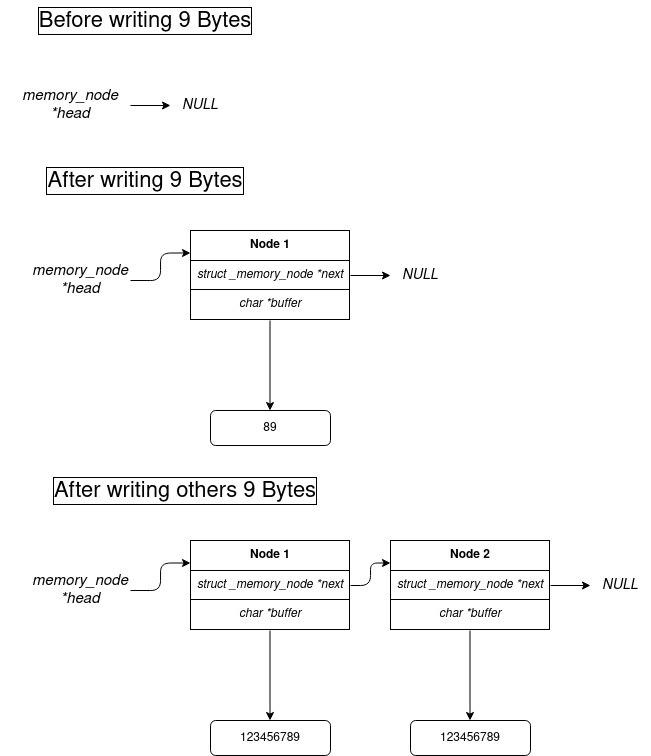
\includegraphics[scale = .45]{write.jpg}
	\caption{Example of write operation}
	\label{fig:write}
\end{figure}




\section{Read Operation}
\label{chap:read operation}

Read operations are all performed synchronously (without delayed work as for write op.), when an invocation occurs the data structure for one of the two flows is set:

\begin{lstlisting}
//FILE: multi_flow.c
if (session->priority == HIGH_PRIORITY){
	priority_obj = &the_object[HIGH_PRIORITY];	
	//...
}else{
	priority_obj = &the_object[LOW_PRIORITY];
	//...
}
ret = read(priority_obj, buff, off, len, session, minor);
\end{lstlisting}

In addition, they involved deleting the bytes read by the user, on the current flow. To do this a linked list was used, in which each node keeps the following fields:

\begin{lstlisting}
//FILE: info.h
typedef struct _memory_node{
	char *buffer;
	struct _memory_node *next;
} memory_node;
\end{lstlisting}

Each node points to its own buffer, the size of which can then be different for all items in the linked list. Buffers are allocated in write operations (see Chap.\ref{chap:write operation}). If the user requests the reading of a smaller number of bytes, than those written on all nodes, the deletion happens for the read bytes only and not on the entire buffer (see Fig.\ref{fig:read}). Reading begins from the first written node (\textbf{First-in-First-out policy}). 

\begin{figure}[h]
	\centering
	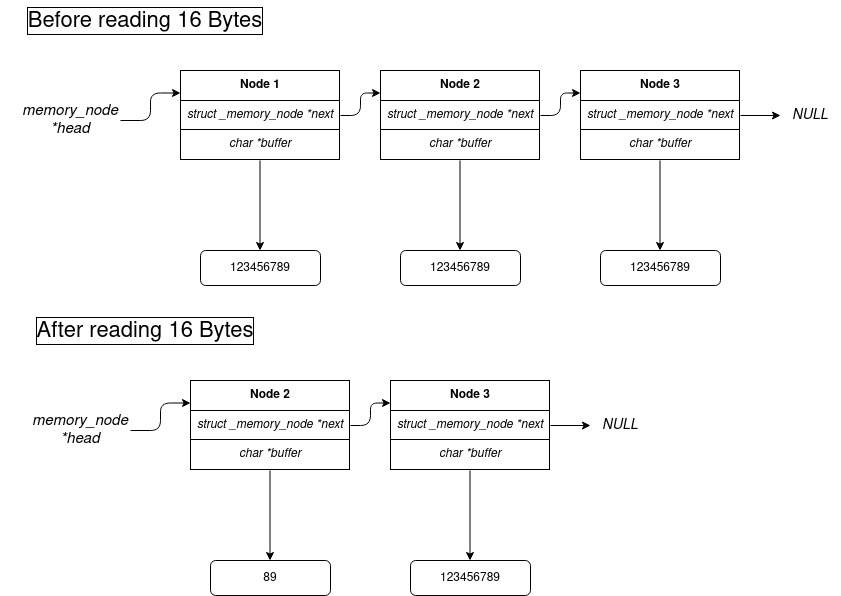
\includegraphics[scale = .45]{read.jpg}
	\caption{Example of read operation}
	\label{fig:read}
\end{figure}

The procedures for doing this are:

\begin{lstlisting}
//FILE: read.h
memory_node *shift_buffer(int, int, memory_node *);
int read(object_state *, const char *, loff_t *, size_t, session *, int);
\end{lstlisting}

\chapter{Parameters}

The required module parameters to deploy are:

\begin{enumerate}
	\item enable or disable the device file
	\item number of bytes currently present in the two flows (high vs low priority)
	\item number of threads currently waiting for data along the two flows (high vs low priority)
\end{enumerate}
implemented with:

\begin{lstlisting}
//FILE: info.h
static bool enabled_device[MINORS];
module_param_array(enabled_device, bool, NULL, 0744);
MODULE_PARM_DESC(...);

static int hp_bytes[MINORS];
module_param_array(hp_bytes, int, NULL, 0744);
MODULE_PARM_DESC(...);

static int lp_bytes[MINORS];
module_param_array(lp_bytes, int, NULL, 0744);
MODULE_PARM_DESC(...);

static int hp_threads[MINORS];
module_param_array(hp_threads, int, NULL, 0744);
MODULE_PARM_DESC(...);

static int lp_threads[MINORS];
module_param_array(lp_threads, int, NULL, 0744);
MODULE_PARM_DESC(...);
\end{lstlisting}



\chapter{User}
\chapter{Reference}
\end{document}          
